% 使用したTeXの種類とバージョン         
% 使用したsice.clsファイルのバージョン  
% 追加したマクロファイル名              
% 印刷したプリンタ名と計算機名          

%%%
%% 和文と英文の2つのテンプレート
%%%  v1.1 [2012/09/05]
%% 1. 和文テンプレート
%% jis.tfm がない場合は,オプションの usejistfm を削除すること
\documentclass[usejistfm]{sice}
%\documentclass[Shortpaper,usejistfm]{sice}
%\documentclass[Technicalnote,usejistfm]{sice}
\usepackage{graphicx}
%\usepackage{latexsym}
%\usepackage[fleqn]{amsmath}
%\usepackage[psamsfonts]{amssymb}
%\usepackage{amsbsy}

\usepackage{amsmath,amssymb,epsf}
\usepackage{algorithm,algorithmic}

\def\R{{\Bbb R}}
\def\N{{\Bbb N}}
\def\Z{{\Bbb Z}}
\def\vec#1{\mbox{\boldmath$#1$}}
\def\sgn#1{\mbox{sgn($#1$)}}
\def\argmin#1{\underset{#1}{\mbox{argmin~}}}
\def\argmax#1{\underset{#1}{\mbox{argmax~}}}
\def\min#1{\underset{#1}{\mbox{min~}}}
\def\max#1{\underset{#1}{\mbox{max~}}}

\def\Underline{\setbox0\hbox\bgroup\let\\\endUnderline}
\def\endUnderline{\vphantom{y}\egroup\smash{\underline{\box0}}\\}
\def\|{\verb|}
\setcounter{page}{1}


%% <local definitions>
%% </local definitions>

\begin{document}
%\specialissue{}
%\Vol{}
%\No{}
%\Year{}
\jtitle{超関数によるノイズにロバストな高速周波数推定}
\jsubtitle{}
\etitle{Robust and Fast Frequency Estimation by Distribution and Kalman Filter}
\esubtitle{}

\authorlist{%
 \authorentry{新田 益大}{Masuhiro Nitta}{KIT}
 \authorentry{西田 健}{Takeshi Nishida}{KIT}
 \authorentry{泉 博之}{Hiroyuki Izumi}{SAN}
}
%\affiliate[ラベル]{日本語所属}{英文所属}
\affiliate[KIT]{九州工業大学大学院工学研究院機械知能工学研究系知能制御工
学部門}{Control Engineering Section, Department of Mechanical and
Control Engineering, Faculty of Engineering, Kyushu Institute of Technology}
\affiliate[SAN]{産業医科大学}{}
%\subtitlenote{○○講演会で発表(2012・4)}

%\received{2012}{1}{1}
%\revised{2012}{1}{1}

\begin{abstract}
 We propose a novel rapid and highly precise frequency estimation
 method of vital signs.
 %
 The proposed method bases on a notion of distribution theory, and  
 is mathematically stable.  
 %
 The proposed method has adaptation ability and shortens the estimation
 time of the conventional method, such as FFT, dramatically. 
% 英文要旨
\end{abstract}
\begin{keywords}
 fast frequency estimation, distribution method, kalman filter
\end{keywords}
\maketitle

\section{はじめに}
%
周波数解析には,振動現象の周波数解析技術が用いられ,ノイズ低減を始めとす
る高速かつ高精度の振動周波数の推定のための手法は数多く提案されている.
%
一般に広く利用される技術としては高速フーリエ変換(FFT: fast Fourier
transform)による信号のスペクトル密度のピーク探索である.
%
これは,一定時間信号を累積するための窓関数を準備し,その区間の信号におけ
る最も支配的な周波数を探索する手法である.
%
しかし,推定周波数の数倍の幅の窓関数を用意する必要があるため,信号の周波
数が低い場合には,数解析結果が算出されるまでの計測時間も長くなる.

一方,近年,超関数を利用する高速かつ高精度の周波数推定手法が提案されてい
る\cite{SF}.
%
本手法による周波数推定は,最低で20サンプリングのデータで高精度の周波数推
定に達成されることが報告されており\cite{SF},振動現象を発生する電子回路
において,その有効性が実証されている.
%
本研究では,この超関数に基づく周波数推定手法に関して,ノイズに対するロバ
スト性を向上させるための手法を提案する.


\section{超関数による周波数推定の概要}
\subsection{定式化}
次のような単周期信号を考える.
\begin{align}
 x(t)=X_0\cos (\omega t- \theta)
\label{eq:a}
\end{align}
ここで,$X_0$は振幅,$\omega$は各周波数,$\theta$は位相の遅れ角であると
する.
%
まず,この信号の2階の微分方程式は以下のように表せる.
\begin{align}
 \ddot{x}(t)+\omega^2x(t)=0
\label{eq:b}
\end{align}
この関係より,周波数は次のように表現できる.
\begin{align}
 \omega^2=\ddot{x}(t)/x(t)
\label{eq:c}
\end{align}
しかし,実応用における離散計測値から$\ddot{x}(t)$を高精度に求め
ることは困難であるため,この関係式を利用する周波数推定は一般に行われない.
同様に,以下の積分の関係を利用する場合も,初期値$x(0)$と$\dot{x}(0)$を高
精度に計測することは困難である.
\begin{align}
x(t)-x(0)-\dot{x}(0)t+\omega^2\int^t_0\int^{t'}_0x(t'') \mbox{d}t''\mbox{d}t'=0
\label{eq:d}
\end{align}

そこで,次のような超関数を利用するパラメータ推定手法を導入する.
まず,パラメータを推定する対象の関数を$f(t)$,
%\begin{align}
% \int_{-\infty}^{\infty}f(t)\phi(t)\mbox{d}t
%\end{align}
%ここで$f(t)$は超関数,
テスト関数$\phi(t)$とおく.
テスト関数は$C^{\infty}$級関数であり,台がコンパクト,すなわち
\begin{align}
 \lim_{t\to \pm \infty}\frac{\mbox{d}^n\phi(t)}{\mbox{d}t^n} = 0\ \ (n=0,1,2,\cdots)
\end{align}
という性質を満たす関数である.
これらの関数の組み合わせにおいて次式が成立する.
\begin{align}
 \int_{-\infty}^{\infty} \frac{\mbox{d} f(t)}{\mbox{d}t}
 \phi(t)\mbox{d}t 
 &=\left[f(t)\phi(t) \right]_{-\infty}^{\infty} -\int_{-\infty}^{\infty} f(t) \frac{\mbox{d} \phi(t)}{\mbox{d}t}
 \mbox{d}t\nonumber\\
 &=-\int_{-\infty}^{\infty} f(t) \frac{\mbox{d} \phi(t)}{\mbox{d}t} \mbox{d}t
\end{align}
したがって,一般に以下が成り立つ.
\begin{align}
 \int_{-\infty}^{\infty} \frac{\mbox{d}^n f(t)}{\mbox{d}t^n}
 \phi(t)\mbox{d}t
 = (-1)^n  \int_{-\infty}^{\infty} f(t) \frac{\mbox{d}^n \phi(t)}{\mbox{d}t^n}
 \mbox{d}t
\label{eq:88}
\end{align}
%
ここで,再び式(\ref{eq:b})の微分方程式を考える.
両辺に$\phi(t)$を乗じて$(-\infty,\infty)$で積分すると,
\begin{align}
 \int_{-\infty}^{\infty}\ddot{x}(t)\phi (t) \mbox{d}t+
 \omega^2 \int_{-\infty}^{\infty}x(t)\phi (t)\mbox{d}t=0
\end{align}
となる.
これは式(\ref{eq:88})に従うと,
\begin{align}
 \int_{-\infty}^{\infty}x(t)\ddot{\phi} (t) \mbox{d}t+
 \omega^2 \int_{-\infty}^{\infty}x(t)\phi (t)\mbox{d}t=0
\end{align}
と変形される.したがって,
\begin{align}
\omega^2=-\frac{
 \int_{-\infty}^{\infty}x(t)\ddot{\phi} (t) \mbox{d}t}{
  \int_{-\infty}^{\infty}x(t)\phi (t)\mbox{d}t}
\label{eq:8}
\end{align}
となる.

次に,ガウス関数は近似的に台がコンパクトであるとみなせるため,テスト関数として
利用することができる.
すなわち,テスト関数を以下のようにおく.
\begin{align}
\phi(t)=\frac{1}{\sqrt{2\pi \sigma^2}}\exp \left\{-\frac{(t-\mu)^2}{2\sigma^2}\right\}
\label{eq:gauss}
\end{align}
ここで$\mu$は平均,$\sigma^2$は分散である.
この二階の導関数は以下のように表せる.
\begin{align}
%\dot{\phi}(t)&=-\frac{t-\mu}{\sigma^2}\phi(t)\\
\ddot{\phi}(t)&=\frac{(t-\mu)^2-\sigma^2}{\sigma^4}\phi(t)
\label{eq:gaussddot}
\end{align}
したがって,式(\ref{eq:gauss})と式(\ref{eq:gaussddot})を利用することで,
式(\ref{eq:8})の$\omega^2$を導出できる.
%
しかし,上述のようにガウス関数を台がコンパクトな関数であると近似するため
には,実応用における計測のサンプリングおよび量子化を考慮する必要がある.

\subsection{推定式の離散化}

テスト関数$\phi(t)$の中央値を$\mu=NT_s/2$と定め,十分に小さな正の実数
$\epsilon$で抑えることができるような$\sigma^2$を設定して
\begin{align}
0< \vert \phi(T_0) \vert=\vert \phi(T_0+NT_s)\vert\ll
\epsilon
\end{align}
と定め,次のように近似する.
\begin{align}
 \int^{\infty}_{-\infty}x(t)\phi(t)\mbox{d}t \simeq 
 \int^{T_0+2\mu}_{T_0}x(t)\phi(t)\mbox{d}t 
\label{eq:appro}
\end{align}
ここで,$N\in \Z_{+}$は任意のサンプリング数,$T_s$はサンプリング周期,
$T_0$は任意の計測開始時刻である.

次に,$x(t)$が離散信号$x(kT_s)$として計測される状況を考え,有限時間$[T_0,
T_0+NT_s]$における式(\ref{eq:8})の算出について考える.
これらの表現を用いると,式(\ref{eq:appro})は区分求積法により以下のように
近似できる.
\begin{align}
 \int^{T_0+2\mu}_{T_0}  x(t)\phi(t)\mbox{d}t  \simeq
 \sum^{N}_{n=0} x(T_0+nT_s)\phi(T_0+nT_s)T_s
\end{align}
これより式(\ref{eq:8})は次のように近似できる.
\begin{align}
\omega^2&\simeq -\frac{\sum^{N}_{n=0}
 x(T_0+nT_s)\ddot{\phi}(T_0+nT_s)}{\sum^{N}_{n=0}
 x(T_0+nT_s)\phi(T_0+nT_s)}
\end{align}
%
ここで,この式は信号の位相に対して不変であることから,式(\ref{eq:a})
の$\theta$に対して不変な推定が行われる.
また,$T_0\geq0$は任意に設定できる.
これらの事実から,次の関係式が成り立つ.
\begin{align}
\omega^2&\simeq -\frac{\sum^{N}_{n=0}
 x(T_0+nT_s)\ddot{\phi}(T_0+nT_s)}{\sum^{N}_{n=0}
 x(T_0+nT_s)\phi(T_0+nT_s)}\nonumber\\
&= -\frac{\sum^{N}_{n=0}
 x(T_0+nT_s)\ddot{\phi}(nT_s)}{\sum^{N}_{n=0}
 x(T_0+nT_s)\phi(nT_s)}\nonumber\\
&= -\frac{\sum^{N}_{n=0}
 x(nT_s)\ddot{\phi}(nT_s)}{\sum^{N}_{n=0}
 x(nT_s)\phi(nT_s)}
\label{eq:omega2}
\end{align}
すなわち,$\phi(t)$および$\ddot{\phi}(t)$は時間更新する必要はな
く,時間$[0, NT_s]$における値を利用し続ければよいことが分かる.
さらに,定数成分を約分して整理すると,次のように表せる.
\begin{align}
\omega^2&\simeq 
-\frac{\sum^{N}_{n=0}x(T_0+nT_s)
 \exp\left\{-\frac{(nT_s-\mu)^2}{2\sigma^2}\right\}\frac{(nT_s-\mu)^2-\sigma^2}{\sigma^4}}
{\sum^{N}_{n=0}x(T_0+nT_s)
 \exp\left\{-\frac{(nT_s-\mu)^2}{2\sigma^2}\right\}
 }\nonumber\\
 &= -\frac{\sum^{N}_{n=0}x_np_nq_n}{\sum^{N}_{n=0}x_np_n}
\label{eq:omega3}
\end{align}
%
%したがって式(\ref{eq:omega2})は,式(\ref{eq:gaussddot})と信号系列をまと
%めたベクトル形式によって以下のように表現できる.
%\begin{align}
%\omega 
%&=\sqrt{
% \sigma^2-
% \frac{\mathbf{q}^T\vec{x}(T_0)}
% {\mathbf{p}^T\vec{x}(T_0)}
% }\biggl/\sigma^2
%\end{align}
ここで,
\begin{align*}
 x_n&\triangleq x(T_0+nT_s)\\
%
 p_n&\triangleq \exp\left\{-\frac{(nT_s-\mu)^2}{2\sigma^2}\right\}\\
%
 q_n&\triangleq \frac{(nT_s-\mu)^2-\sigma^2}{\sigma^4}
\end{align*}
であり,$x_n$は周波数が変化する場合を考慮して$T_0$に関して時変とする.
したがって,$x_n$が全て発生するまでの時間$[0,NT_s]$は,$\omega$
の推定は実行されないことに注意が必要である.
また,時刻$NT_s$以降はFIFO形式で$x_n$の要素をシフトしながら更新する.
%
さらに,先行研究における解析から,$N$および$\sigma$,$T_s$
は次の関係を満たすように設定する必要があることが明らかにされている.
\begin{align}
 20T_s \leq 16\sigma < NT_s
\end{align}
多くの事例では$T_s$は計測機器に依存して変更できないため,$N$を定めた後に,
上述の関係を満たす範囲で$\sigma$を定めれば良い.
すると,$p_n$と$q_n$は計測と無関係であるため,上述のパ
ラメータがが決定されれば直ちに設定される.

以上より明らかなように,本手法は最低限で連続する20のサンプリング時刻におけ
る計測値が獲得できれば,周波数推定が実行可能である.
%
さらに,振動の周波数が変動する場合にも,$\vec{x}(T_0)$を逐次更新すること
で推定を適応的に修正することが可能である.

一方,時系列計算を行なっている最中に以下のような状況においては推定精度が低下
することに注意が必要である.
\begin{align}
 \frac{\sum^{N}_{n=0}x_np_nq_n}{\sum^{N}_{n=0}x_np_n}&>0\\
 \sum^{N}_{n=0}x_np_n&<\varepsilon \ \ (\mbox{e.g.}\  \varepsilon=10^{-6})
\end{align}
これらの場合には,前時刻の推定を継続して利用するなど,推定の不安定化を回
避する方策を設ける必要がある.


\section{シミュレーション}

%
%ヒトの呼吸数をこの関係で表す場合には,$X_0$および$\omega$,$\theta$は時
%変関数で表す必要があるが,定式化においては時不変の定数として扱い,後にこ
%れらの変動に適応する機構を考慮する.

ここでは,次の信号を用いて上述の推定手法の性能をシミュレーションにより検
証する.
\begin{align}
 x(t)=\cos(0.5\pi kT_s+\pi/2)
\end{align}
ここで$T_s=0.01$[s]および$N=20$と定め,$\sigma$をそれらの従属変数として
定めるために,以下の関数を設けた.
\begin{align}
\sigma=((N-20)/2+20)T_s/4
\end{align}

まず,以上の条件におけるテスト関数$\phi(t)$とその2階微分
$\ddot{\phi}(t)$の概形を図\ref{fig:ddphi}に示す.
\begin{figure}[bp]
 \begin{center}
  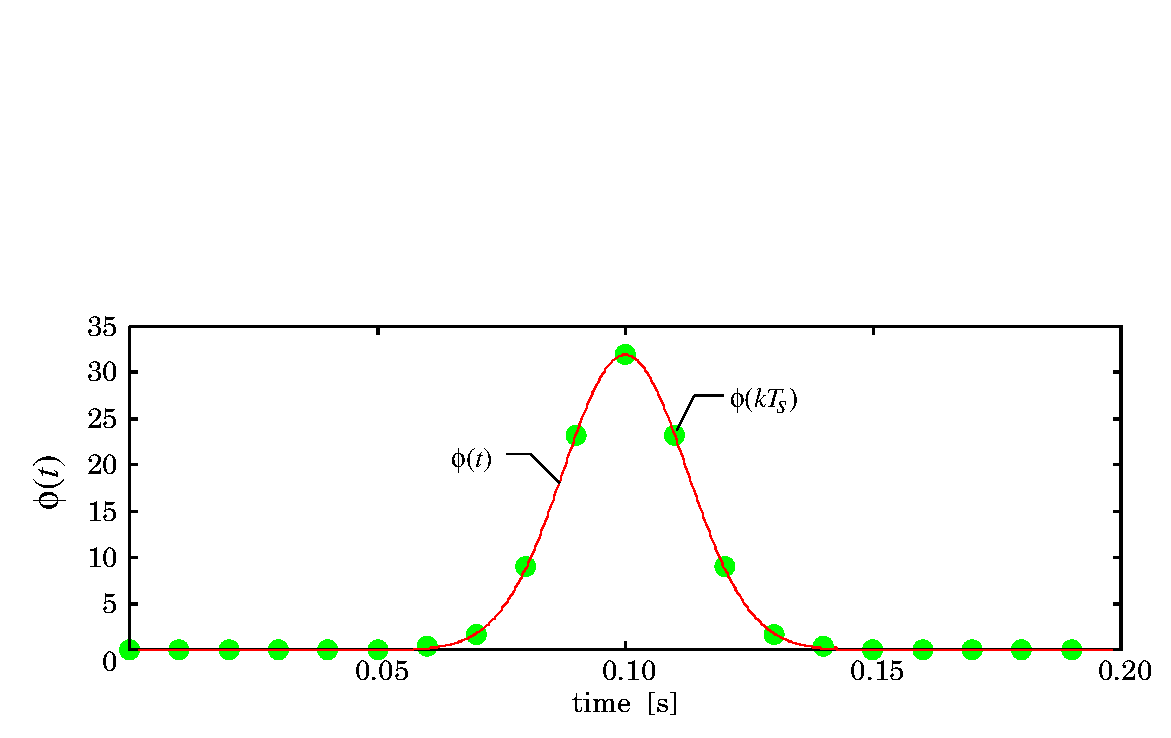
\includegraphics[width=1.0\linewidth]{fig/phi2.eps}\\
  (a) $\phi(k)$\\
  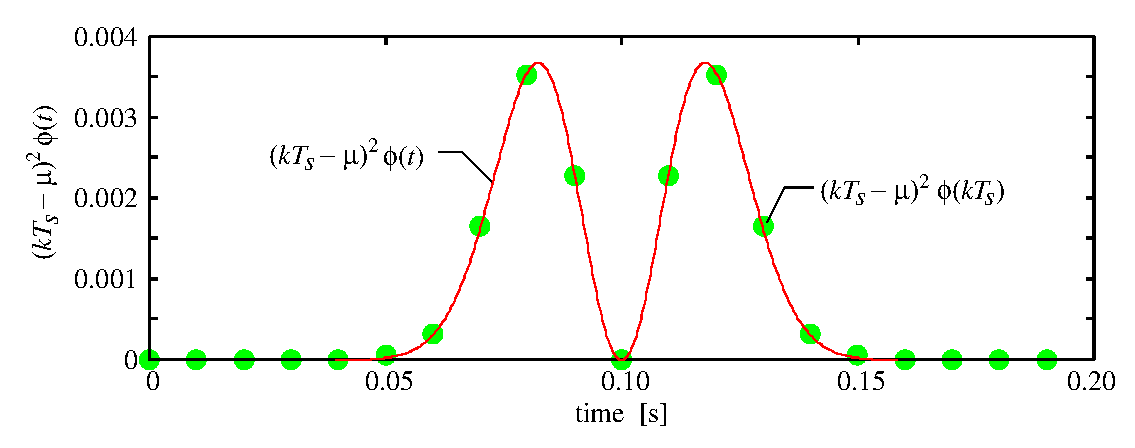
\includegraphics[width=1.0\linewidth]{fig/ddphi2.eps}\\
  (b) $\ddot{\phi}(k)$
 \end{center}
 \caption{The test function of $\mathbf{p}$ and $\mathbf{q}$ ($N=21$).}
 \label{fig:ddphi}
\end{figure}
さらに,それらを利用して推定した結果を図\ref{fig:sim2}に示す.
\begin{figure}[btp]
 \begin{center}
  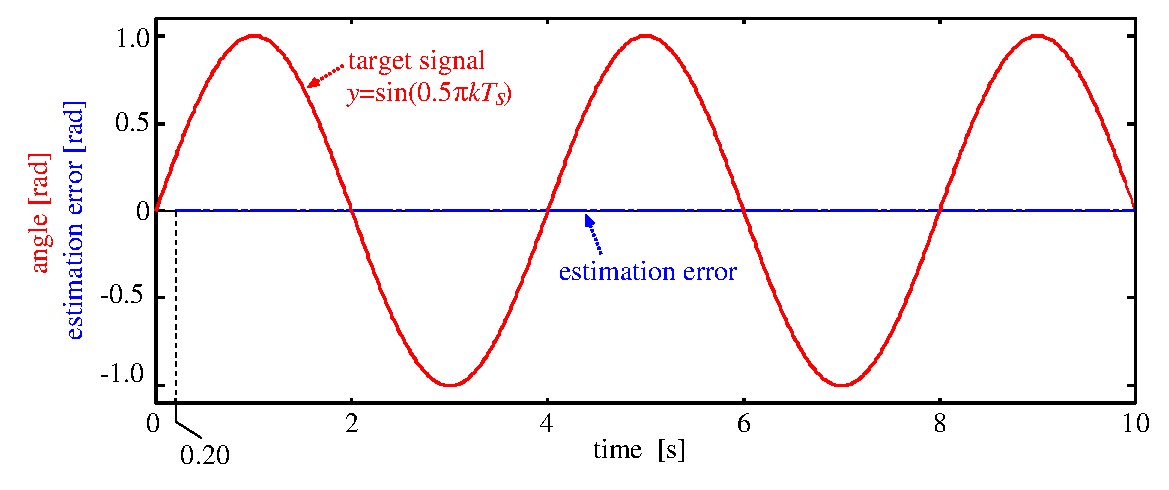
\includegraphics[width=1.0\linewidth]{fig/sim2.eps}
 \end{center}
 \caption{A periodic signal and its frequency estimation results.}
 \label{fig:sim2}
\end{figure}
推定が開始される時刻0.21[s]以降は推定誤差が0であった.
この結果より,単一周期の信号の推定が本手法によって実現されることが示され
た.





\section{おわりに}

%\begin{acknowledgment}% 謝辞
%\end{acknowledgment}

\begin{thebibliography}{}
 \bibitem{SF} A. Ishizaka, M. Nitta, K. Koto, ``Error analysis on
	 distribution-based frequency estimator'', Proc. of
	 Int. Conf. on Control, automation, and Systems, pp. 255--260, 2010.

 \bibitem{Ni} 新田益大, ``超関数に基づく高精度周波数推定'', 第12回計測自
	 動制御学会制御部門大会, 2012.

\end{thebibliography}

%\appendix
%\section{}

\begin{biography}
\profile{m}{新田 益大}{
平24年より九工大・機械知能工学・助教,博士(工学).
}

\profile{m}{西田 健}{
平10九工大・工・設計生産工卒.
平14九工大大学院博士後期課程修了.同年より九工大・機械知能工学・助手.平
成25年より准教授,博士(工学).屋外移動ロボットに関する研究に従事.日本ロ
ボット学会,計測自動制御学会,日本神経回路学会,電子情報通信学会などの会員.
}

\profile{n}{泉 博之}{
産医大・准教授
}

\end{biography}

\end{document}


%% 英文テンプレート
\documentclass[English]{sice}
%\documentclass[Shortpaper,English]{sice}
%\documentclass[Technicalnote,English]{sice}
\usepackage{graphicx}
%\usepackage{latexsym}
%\usepackage[fleqn]{amsmath}
%\usepackage[psamsfonts]{amssymb}
%\usepackage{amsbsy}

\setcounter{page}{1}

%% <local definitions>
%% </local definitions>

\begin{document}
%\specialissue{}
%\Vol{}
%\No{}
%\Year{}
\etitle{}
\esubtitle{}

\authorlist{%
 \authorentry{}{}
}
\affiliate[]{}

%\titlenote{}
%\subtitlenote{}

%\received{2012}{1}{1}
%\revised{2012}{1}{1}

\begin{abstract}% 英文要旨
\end{abstract}
\begin{keywords}% 英文キーワード
\end{keywords}
\maketitle

\section{Introduction}


\begin{acknowledgment}% 謝辞
\end{acknowledgment}

\begin{thebibliography}{99}% 文献が10以上のとき99,10未満のとき9
\bibitem{}
\end{thebibliography}

\appendix
\section{}

\begin{biography}
\profile{}{}{%
}
\end{biography}

\end{document}

